\chapter{Versuchsaufbau und -ablauf}\label{Kapitel 3}
\interfootnotelinepenalty 10000
Das folgende Kapitel beschreibt Versuchsaufbau und -durchf"uhrung sowie Ziele der Messung, von der Erkenntnisse "uber das Skalierungsverhalten eines RPi-Clusters unter der Workload der ausgew"ahlten HPC-Benchmarks erwartet werden. 

\section{Zielsetzung}

F"ur das Skalierungsverhalten des Bramble unter der Workload von Linpack und STREAM wird wie in Kap. \ref{Leistung} beschrieben die Time to Completion als ausschlaggebende Ma\ss zahl betrachtet. Die ausgew"ahlten Benchmarks Linpack, Whetstone und STREAM werden zun"achst auf einem vom RPi-Cluster unabh"angigen RPi-Einzelrechner ausgef"uhrt. Dann wird versucht, sie in einer passenden MPI-Implementierung auf dem Bramble lauff"ahig zu machen. Anschlie\ss end erfolgt eine Gegen"uberstellung mit den Ergebnissen der Benchmark-Autoren (vgl. Kap. \ref{vergleich}) und denen tats"achlicher Supercomputer (vgl. Kap. \ref{top500}).

Alle Messungen werden auf 1 -- n RPi-Nodes des Bramble mit n=19 RPi-Nodes (vgl. Kap. \ref{Zugriff}). Alle Messungen werden zweimal durchgef"uhrt: Mit Netzwerkanschluss der nicht beteiligten RPi-Nodes an \texttt{careme} und ohne. F"ur beide Benchmarks werden zwei Ergebnisparameter betrachtet: Ausf"uhrungsrate in GFLOPS und Ausf"uhrungszeit in s f"ur HPLinpack, Ausf"uhrungsrate in MB/s und durchschnittliche Ausf"uhrungszeit in s f"ur STREAM. Die Ergebnisse mit und ohne Netzwerkanschluss der nicht beteiligten RPi-Nodes werden anschlie\ss end gegen"ubergestellt (vgl. Kap. \ref{Ergebnisse}). 

Der Schwerpunkt der Untersuchung liegt auf dem Bramble. Da sich seine Systemarchitektur wie in Kap. \ref{Bramble-Spezi} erl"autert stark von einem RPi-Einzelrechner unterscheidet und unterschiedliche Implementierungen der Benchmarks verwendet werden, k"onnen die Ergebnisse des RPi-Einzelrechner lediglich als grobe Richtlinie dienen.  

\section{Aufbau und Art der Messung}\label{Aufbau}

Hier stellen sich zwei grunds"atzliche Fragen: Welcher Art ist die Messung und welche Voraussetzungen sind daf"ur erforderlich? 

Die Time to Completion wird pro Benchmark durch zwei zeitabh"angige Ausgabeparameter gemessen. Drei Versuchsszenarien kommen zur Anwendung: RPi-Einzelrechner, Bramble mit 19--1 RPi-Nodes aktiv/19 powered, Bramble mit 19--1 RPi-Nodes aktiv/19--1 RPi-Nodes powered. 

F"ur den Versuchsaufbau sind daher folgende Aspekte von Bedeutung: M"ogliche Modifikationen der RPi-Nodes (Hardware, OS-Konfiguration), Zeitsynchronisation der RPi-Nodes, Skalierung der Messung auf 19--n RPi-Nodes, automatisierte Durchf"uhrung der Messung auf 19--n RPi-Nodes sowie Einlesen der Messwerte in eine geeignete Datenstruktur. 

\subsection{Versuchsaufbau Ri-Einzelrechner}\label{RPi-Versuchsaufbau}

F"ur die meisten User eines RPi-Einzelrechners stellt sich nach Auswahl, Installation und Konfiguration des Betriebssystems die Frage nach Swap Space und "Ubertakten. Beides liegt auf der Hand, da das Modell B des RPi nur "uber 512 MB Arbeitsspeicher verf"ugt. Die CPU-Leistung ist mit 700 MHz ebenfalls eher niedrig. 

Im Praxisbetrieb zeigte sich, dass ein "Ubertakten der CPU auf bis auf 1 GHz gefahrlos m"oglich ist. Beim hier verwendeten Testger"at wurde darauf verzichtet, um die Vergleichbarkeit mit den Versuchsergebnissen des Bramble nicht zu gef"ahrden\footnote{Es erscheint wenig zielf"uhrend, die Komponente zu tunen, deren Performance man durch Benchmarking evaluieren m"ochte. F"ur eine sp"atere Untersuchung ist dies jedoch nicht ausgeschlossen. Z.B. w"are es interessant zu ermitteln, ob man den relativ hohen Stromverbrauch des Bramble bei Niedriglast (vgl. \cite{kli13}) durch Untertakten der einzelnen CPUs senken kann. Ergebnisse f"ur Linpack 100 und Whetstone bei "Ubertakten der CPU auf 1 MHz wurden bereits ver"offentlicht (vgl. \url{http://www.roylongbottom.org.uk/Raspberry\%20Pi\%20Benchmarks.htm}).}.

Das gew"ahlte Betriebssystem Raspbian verwendet standardm"a\ss ig eine Swap-Datei \texttt{/var /swap}, die den Adressraum des Arbeitsspeichers bei "Uberlast erweitert. Hierbei gibt es zwei Probleme: Erstens k"onnen st"andige Schreibzugriffe auf Dauer die SD-Karte besch"adigen\footnote{Vgl. \cite{pow12}.}, zweitens sind Schreibzugriffe auf die SD-Karte sehr langsam, was die Performance des Systems bei hoher Arbeitsspeicherlast beeintr"achtigen kann. Daher wurde auf die Swap-Datei verzichtet\footnote{Sie kann mit dem Befehl \texttt{sudo update-rc.d dphys-swapfile remove} deaktiviert werden. Eine weitere M"oglichkeit des Swapping ist die Verwendung von zRAM, sodass ein Teil des Arbeitsspeichers komprimiert und als Swap Space genutzt wird (vgl. \cite{pow12}). Die Allokierung einer auf Unix-Systemen "ublicherweise genutzten Swap-Partition ist nicht sinnvoll, da auch hierdurch die Lebensdauer der SD-Karte durch h"aufige Schreibzugriffe verk"urzt wird.}. 

Die Zeitsynchronisation des RPi erfolgt beim Booten durch Abgleich mit einem NTP-Server. Da er nicht mit weiteren Nodes oder einem zentralen Server synchronisiert werden muss, er"ubrigt sich hier eine weitere Zeitsynchronisation. Skalierung der Messung und automatisierte Durchf"uhrung sind ebenfalls nur f"ur den Bramble von Bedeutung. Auf das Einlesen der Werte in die Datenbank des Bramble wurde auf Grund des unterschiedlichen Versuchsaufbaus ebenfalls verzichtet. 

\subsection{Versuchsaufbau Bramble}\label{Bramble-Versuchsaufbau}

Das folgende Komponentendiagramm \ref{fig:Komponentendiagramm} zeigt den Versuchsaufbau pro Messreihe auf dem Bramble, der als \textit{ExperimentSuite} bezeichnet wird. Es enth"alt die systemkritischen Elemente des Versuchsaufbaus: Stromversorgung und Netzanschluss des Bramble als physische Komponenten sowie die MySQL-Datenbank \texttt{rpiWerte} als logische Komponente. Der Bramble wird als "`Black Box"' betrachtet, d.h. es werden keine Messwerte der einzelnen RPi-Nodes, sondern des Clusters als Gesamtsystem betrachtet.  
\begin{figure}[htb]
  \centering
  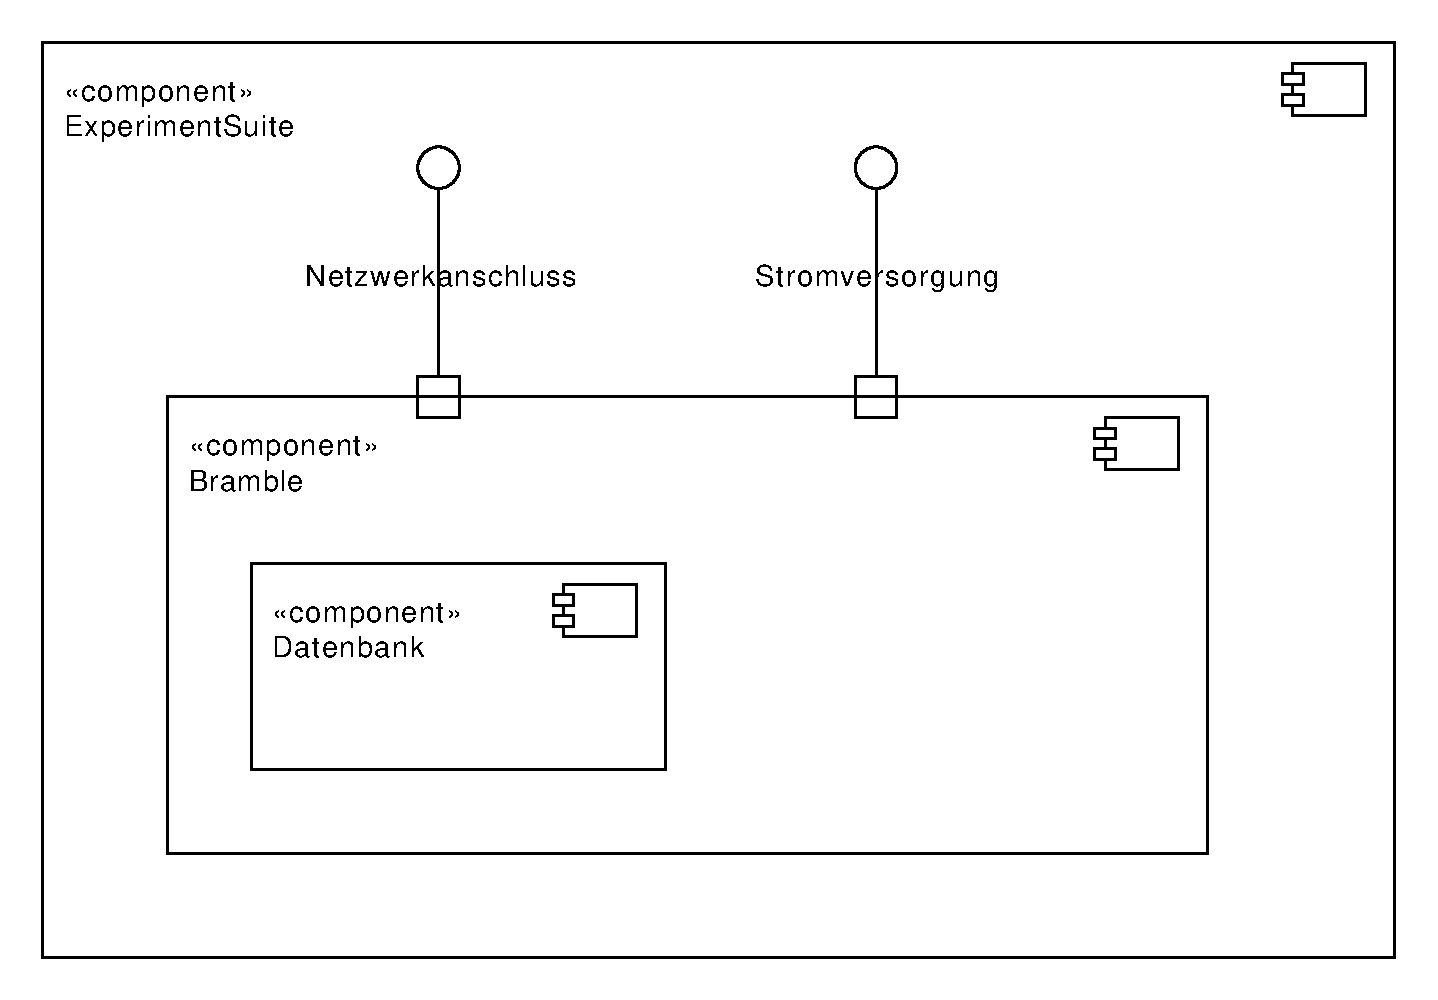
\includegraphics[width=\textwidth]{komponentendiagramm1.pdf}\\ 
  \caption{Komponentendiagramm des Versuchsaufbaus.}
  \label{fig:Komponentendiagramm}		
\end{figure}

\subsubsection{Modifikationen der RPi-Nodes}

Betriebssystem und Filesystem des Bramble wurden so "ubernommen wie bei Beginn der Untersuchung zur Verf"ugung gestellt: Die CPUs der RPi-Nodes sind nicht "ubertaktet und der Bramble-Server \texttt{careme} nutzt keinen Swap Space. Bei den RPi-Nodes war allerdings ein gro\ss er Teil der SD-Karten als Swap Space allokiert worden\footnote{Vgl. \cite{kli13}.}. Im Praxisbetrieb zeigten sich jedoch rasch Schwierigkeiten, die Anpassungen in OS-Konfiguration und Hardware erforderlich machten. Folgende Fehlerf"alle waren am h"aufigsten: 
\begin{enumerate}
	\item \textbf{Defekte Hardware (Mini-USB-Kabel)}\\
Einige Mini-USB-Kabel waren bereits zu Beginn der Untersuchung defekt oder hatten einen Wackelkontakt. Sie mussten durch funktionsf"ahige Kabel ersetzt werden. 
	\item \textbf{RPi-Node nicht erreichbar (\texttt{ping})}\\
H"aufig reagierte ein RPi-Node nicht auf ein \texttt{ping} von einem RPi-Node oder von \texttt{careme} aus (Fehlermeldung \texttt{Destination Host Unreachable}), obwohl die Status-LEDs aktiv waren. Als einzige L"osung erwies sich Ziehen und Wiedereinstecken des Mini-USB-Kabels; war das nicht erfolgreich, musste das Vorgehen mit dem Netzwerkkabel wiederholt werden (das Netzwerkkabel allein reicht nicht aus). Danach war der Host i.d.R. wieder mit \texttt{ping} erreichbar. 
	\item \textbf{RPi-Node nicht erreichbar (SSH)}\\ 
Hier traten drei Fehlerf"alle auf: Am h"aufigsten war die Fehlermeldung \texttt{No route to host} beim Versuch, von \texttt{careme} oder einem anderen RPi-Node aus eine SSH-Verbindung zum Zielhost herzustellen. Die einzige L"osung ist Ziehen und wieder Einstecken des Netzwerkkabels. Nach einigen Minuten ist der Host i.d.R. wieder erreichbar. 

Ein weiterer Fehlerfall war ein "uberraschender Passwortprompt f"ur \texttt{root} beim Versuch, eine SSH-Verbindung zu einem RPi-Node zu einem anderen RPi-Zielnode aufzubauen. Dieses Problem lie\ss sich durch Eintragen des RSA Public Key von 
\texttt{root} in die Datei \texttt{\textasciitilde/.ssh/authorized\_keys} auf dem Zielhost l"osen. 

Seltener trat die Fehlermeldung \texttt{WARNING: REMOTE HOST IDENTIFICATION HAS CHAN\-GED!} auf. Dies konnte durch Korrektur des RSA Public Key des Anfragehosts in der Datei \texttt{\textasciitilde/.ssh/known\_hosts} auf dem Zielhost gel"ost werden. 
	\item \textbf{Geshartes Verzeichnis nicht gemountet}\\
Beim Neustart eines RPi-Nodes oder des gesamten Clusters wurde h"aufig das gesharte Verzeichnis nicht gemountet, was zu Fehlermeldungen wie \texttt{-bash: /srv/libraries/ etc/.sharedprofile: No such file or directory} f"uhrte und sich durch Mounten des Verzeichnisses mit \texttt{mount /srv} beheben lie\ss .
	\item \textbf{bash-Befehle werden nicht erkannt}\\
Aus unklaren Gr"unden wurden manchmal von einzelnen RPi-Nodes h"aufig verwendete bash-Befehle nicht mehr erkannt, was sich an Fehlermeldungen wie \texttt{mpiexec: command not found} zeigt. Latenzen beim Zugriff auf den gemeinsamen Speicherbereich k"onnten der Grund hierf"ur sein, da sich ein Logout und erneuter Login auf dem betreffenden RPi-Node als einzige L"osung erwies. 
\end{enumerate}

\subsubsection{Zeitsynchronisation der RPi-Nodes} 

Ein wichtiger Aspekt bei der parallelen Ausf"uhrung eines Programms auf mehreren Rechnerkernen ist die exakte Zeitsynchronisation. Auf dem Bramble wird die Zeitsynchronisation der RPi-Nodes durch einen auf \texttt{careme} installierten OpenNTP-Server realisiert. Die einzelnen RPi-Nodes synchronisieren sich gegen diesen Server\footnote{Vgl. \cite{kli13}.}. Die Zeitsynchronisation der RPi-Nodes ist somit auch f"ur die verteilte Ausf"uhrung der Benchmarks gew"ahrleistet.

\subsubsection{Skalierung der Messung auf 19--n RPi-Nodes} 

Das folgende Aktivit"atsdiagramm zeigt, welche Schritte aus Benutzersicht f"ur die Durchf"uhr\-ung einer ExperimentSuite, d.h. der Ausf"uhrung eines Benchmarks auf einer gew"ahlten Anzahl von aktiver und powered RPi-Nodes erforderlich sind. Es wird mit n=19 RPi-Nodes begonnen und einmal "uber alle Nodes von 20--1 (ohne den Ausf"uhrungsknoten \texttt{pi03}) iteriert. Danach wird die zweite Messung durchgef"uhrt, wobei nach jedem Iterationsschritt der nicht mehr ben"otigte RPi-Node abgeschaltet wird. Jede Iteration der Benchmark-Ausf"uhrung l"auft prinzipell gleich ab, w"ahrend am Anfang und am Ende spezielle Vorkehrungen zu treffen sind. 
\begin{figure}[htb]
  \centering
  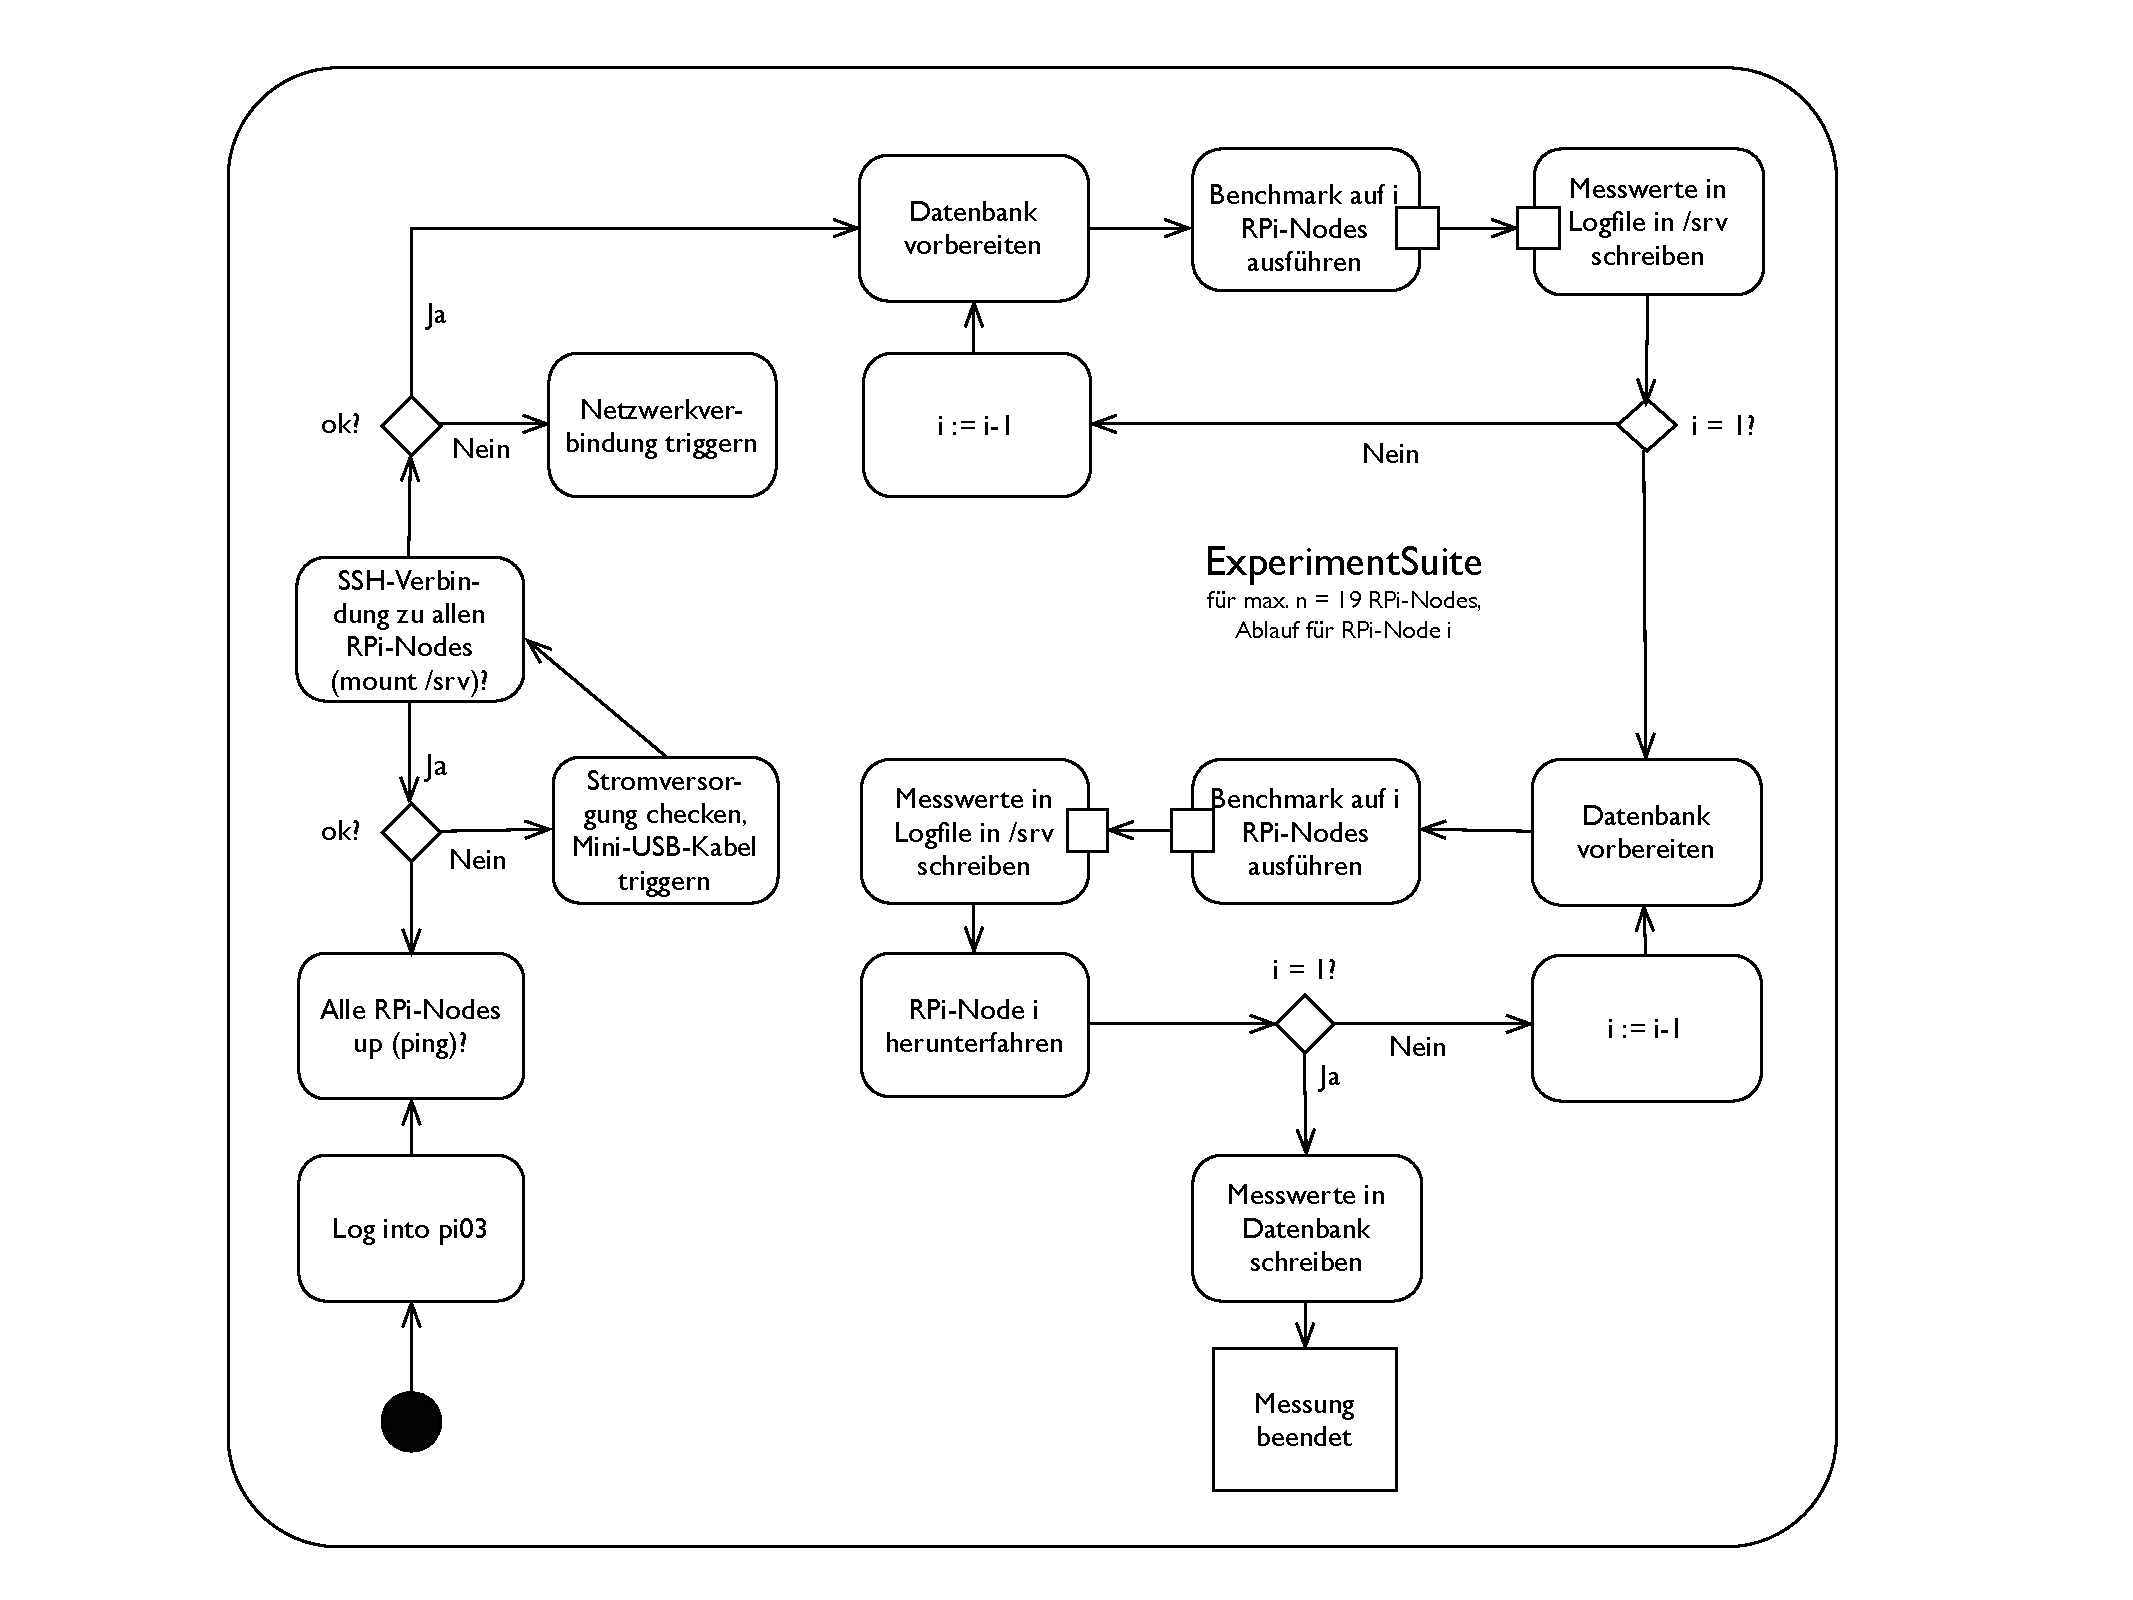
\includegraphics[scale=0.5]{aktivitaetsdiagramm1.pdf}\\ 
  \caption{Aktivit"atsdiagramm der ExperimentSuite.}
  \label{fig:Aktivitaetsdiagramm}
\end{figure}

\subsubsection{Automatisierte Durchf"uhrung der Messung auf 19--n RPi-Nodes} 

Die automatisierte Durchf"uhrung der Messung erfolgt durch Shellskripte. Sie werden im gesharten Verzeichnis abgelegt und k"onnen von \texttt{pi03} oder einem anderen Ausf"uhrungsknoten aus gestartet werden. Folgende Schritte werden durch die Skripte realisiert: 

\begin{enumerate}
	\item Erstellen eines Machinefile zur Verteilung der Workload auf n RPi-Nodes, ggf. L"oschen des alten.
	\item Mounten des gesharten Verzeichnisses auf allen RPis. 
	\item Navigation ins Arbeitsverzeichnis der Experimentsuite. 
	\item Iteration "uber n ausgew"ahlte Benchmarks: 
	\begin{enumerate}
		\item Erstellen der Logfiles. 
		\item Iteration "uber n RPi-Nodes:
		\begin{enumerate}
			\item Einrichten der Datenbank. 
			\item Verteilte Ausf"uhrung des Benchmarks auf n RPi-Nodes. 
			\item Loggen der Ergebnisdaten. 
		\end{enumerate}
		\item Iteration "uber n RPi-Nodes: 
		\begin{enumerate}
			\item Einrichten der Datenbank.
			\item Verteilte Ausf"uhrung des Benchmarks auf n RPi-Nodes. 
			\item Shutdown von RPi-Node n. 
			\item Loggen der Egebnisdaten.   
		\end{enumerate}
		\item Parsen der Logfiles f"ur die Datenbank-Eingabe. 
		\item Schreiben der Messergebnisse in die Datenbank. 
	\end{enumerate}
\end{enumerate}
\noindent
Dazu wurden drei Shellskripte \texttt{startBenchmarks.sh} (Schritte 1--3), \texttt{STREAM.sh} und \texttt{hpl-2.1.sh} (Schritt 4 f"ur den jeweiligen Benchmark) erstellt. Der Quellcode findet sich in \mbox{Kap. \ref{skripte}}.

\subsubsection{Einlesen der Messwerte in eine geeignete Datenstruktur}

Schlie\ss lich stellt sich die Frage, wo und in welcher Form die Ergebnisdaten zweckm"assigerweise abgelegt werden. Die Entscheidung fiel zu Gunsten einer MySQL-Datenbank auf \texttt{careme}. Sie orientiert sich an einem vorgegebenen Datenbankschema, das die Bramble-ExperimentSuites in einen gr"o\ss eren Versuchsaufbau integriert. W"ahrend der praktischen Arbeit wurde das Schema schrittweise an die tats"achlichen Erfordernisse angepasst. Z.B. wurde f"ur jedes ausgef"uhrte Teilmodul eines Benchmarks ein Parameter definiert, der Unix-Timestamp seines Ausf"uhrungsendes ermittelt und zusammen mit dem jeweiligen Messwert in die Datenbank eingelesen.

Um dem gew"ahlten Datenbankschema gerecht zu werden, mussten neben der Tabelle mit den Messergebnissen weitere Tabellen bef"ullt und "uber eine N2M-Tabelle verkn"upft werden (vlg. \ref{fig:Aktivitaetsdiagramm}, "`Datenbank vorbereiten"'): 
\begin{enumerate}
	\item Benennung und Beschreibung des Benchmarks 
	\item Benennung und Beschreibung des Versuchsaufbaus 
	\item Konfiguration des Versuchsaufbaus 
\end{enumerate} 
Im ersten Schritt werden die statischen Konfigurationen f"ur STREAM und HPLinpack festgelegt, was durch zwei weitere Shellskripte \texttt{loadGeneratorConfigHpl.sh} und \texttt{loadGenerator\-ConfigStream.sh} (vgl. Kap. \ref{skripte}) realisiert wurde. Die dynamischen Schritte pro ExperimentSuite (Benennung, Beschreibung und Konfiguration des Versuchsaufbaus, Einlesen der Messwerte und Verkn"upfung von ExperimentSuite mit Benchmark-Konfiguration) wurden in die Ausf"uhrungsskripte der Benchmarks integriert. 

\section{Ergebnisse}\label{Ergebnisse}

Der n"achste Abschnitt pr"asentiert die Untersuchungsergebnisse mit Schwerpunkt auf dem Bramble. F"ur die Durchf"uhrung standen auf Grund der oben beschriebenen Probleme nur 17 RPi-Nodes zuverl"assig zur Verf"ugung. Zur besseren Lesbarkeit der Ergebnisse wurde entschieden, beide Benchmarks auf gleich vielen RPi-Nodes auszuf"uhren. Da HPLinpack mindestens vier Prozessoren bzw. Prozesse ben"otigt, wurde die Anzahl der Prozessoren f"ur STREAM hieran angepasst. Beide Benchmarks wurden demnach auf n=16 RPi-Nodes ausgef"uhrt, \texttt{pi03} dient als Ausf"uhr\-ungsknoten und wird in der Messung nicht ber"ucksichtigt.

\subsection{RPi-Einzelrechner: Linpack 100, Whetstone und STREAM}\label{rpi-ergebnisse}

Bei der Ausf"uhrung von Linpack 100, Whetstone und STREAM in den ausgew"ahlten Implementierungen erreichte der RPi-Einzelrechner folgende Ergebnisse: 

\begin{enumerate}
	\item \textbf{Linpack 100} 
	\begin{itemize}
		\item \textbf{Ausf"uhrungsrate:} 41.31 MFLOPS = 0.04131 GFLOPS
	\end{itemize}
	\item \textbf{Whetstone} 
	\begin{itemize}
		\item \textbf{Ausf"uhrungsrate:} 255.154 MWIPS
		\item \textbf{Ausf"uhrungszeit:} 10.190 s  
	\end{itemize}
	\item \textbf{STREAM} 
	\begin{itemize}
		\item \textbf{Ausf"uhrungsrate:}
		\begin{enumerate}
			\item COPY: 274.4. MB/s
			\item SCALE: 209.3 MB/s
			\item ADD: 287.2 MB/s
			\item TRIAD: 271.1 MB/s
		\end{enumerate}					 
		\item \textbf{Ausf"uhrungszeit:}
		\begin{enumerate}
			\item COPY: 0.586838 s
			\item SCALE: 0.766437 s
			\item ADD: 0.838107 s
			\item TRIAD: 0.886793 s
		\end{enumerate}
	\end{itemize}
\end{enumerate} 
Detaillierte Ergebnisdateien finden sich im Anhang (vgl. Kap. \ref{rpi-anhang}). 
 
\subsection{Bramble: HPLinpack}\label{ergebnisse-hpl}

Die folgenden Diagramme zeigen die Ergebnisse f"ur HPLinpack auf dem Bramble mit zwei Ausgabeparametern: Time to Completion und CPU-Performance in MFLOPS, jeweils skaliert auf 16--4 RPi-Nodes. Diagramme \ref{fig:hpl1} und \ref{fig:hpl2} zeigen die Ergebnisse f"ur n RPi-Nodes aktiv/16 RPi-Nodes powered (d.h. alle). Diagramme \ref{fig:hpl3} und \ref{fig:hpl4} zeigen das Verhalten bei n RPis aktiv/n RPis powered.
\enlargethispage*{2cm}
\begin{figure}[htb]
  \centering
  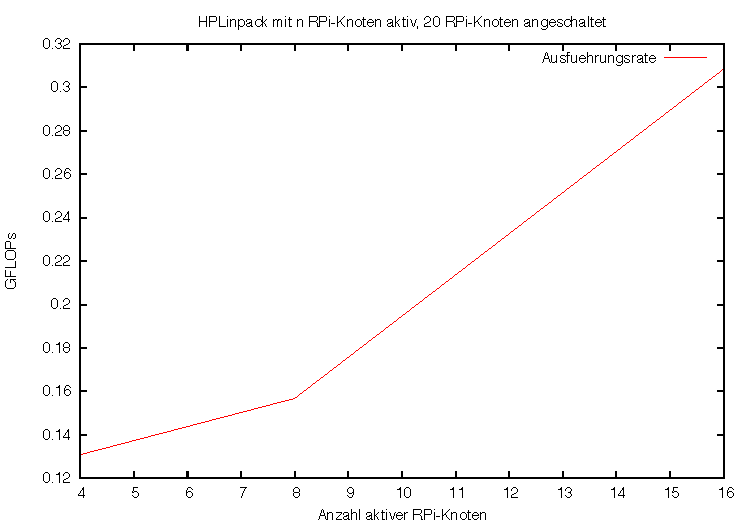
\includegraphics[scale=0.8]{hpl1.pdf}\\ 
  \caption{Ausf"uhrungsrate in GFLOPS f"ur HPLinpack auf n RPi-Nodes aktiv/16 RPi-Nodes powered.}
  \label{fig:hpl1}		
\end{figure}
\begin{figure}[h!]
  \centering
  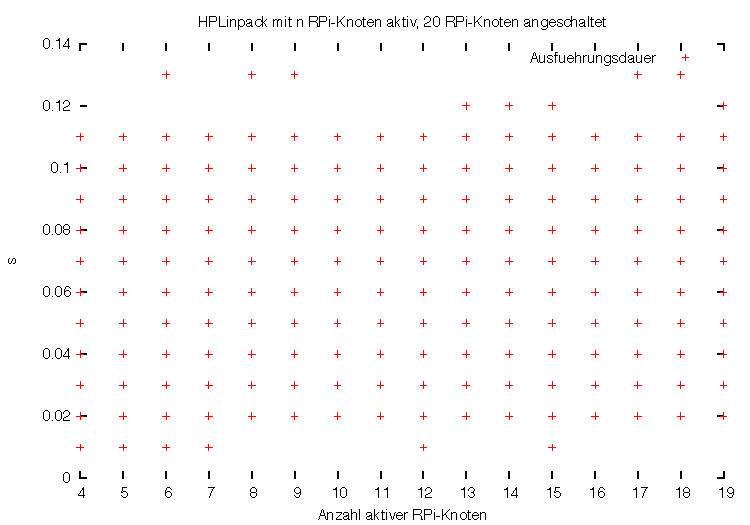
\includegraphics[scale=0.8]{hpl2.pdf}\\ 
  \caption{Ausf"uhrungszeit in s f"ur HPLinpack auf n RPi-Nodes aktiv/16 RPi-Nodes powered.}
  \label{fig:hpl2}		
\end{figure}
\begin{figure}[htb]
  \centering
  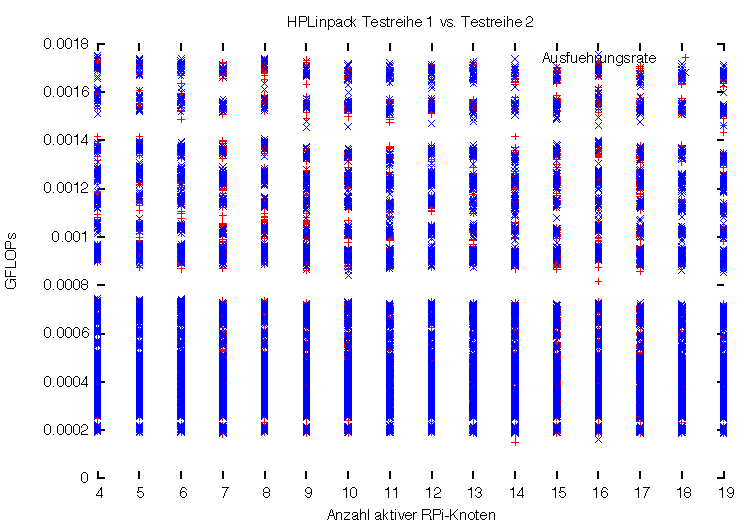
\includegraphics[scale=0.8]{hpl3.pdf}\\ 
  \caption{Ausf"uhrungsrate in GFLOPS f"ur HPLinpack auf n RPi-Nodes aktiv/n RPi-Nodes powered.}
  \label{fig:hpl3}		
\end{figure}
\begin{figure}[h!]
  \centering
  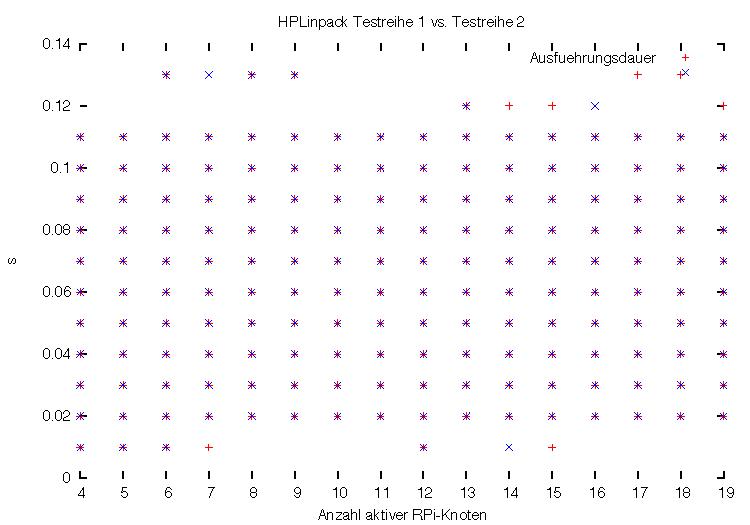
\includegraphics[scale=0.8]{hpl4.pdf}\\ 
  \caption{Ausf"uhrungszeit in s f"ur HPLinpack auf n RPi-Nodes aktiv/n RPi-Nodes powered.}
  \label{fig:hpl4}		
\end{figure}

\newpage
\subsection{Bramble: STREAM}\label{ergebnisse-stream}
Die folgenden Diagramme zeigen die Ergebnisse von STREAM auf dem Bramble f"ur die Module Copy, Scale, Add und Triad, jeweils mit zwei Ausgabeparametern und skaliert auf 16--4 RPi-Nodes. Diagramme \ref{fig:stream1} und \ref{fig:stream2} zeigen die Ergebnisse f"ur n RPi-Nodes aktiv/16 RPi-Nodes powered, Diagramme \ref{fig:stream3} und \ref{fig:stream4} f"ur n RPi-Nodes aktiv/n RPi-Nodes powered. 

\begin{figure}[htb]
  \centering
  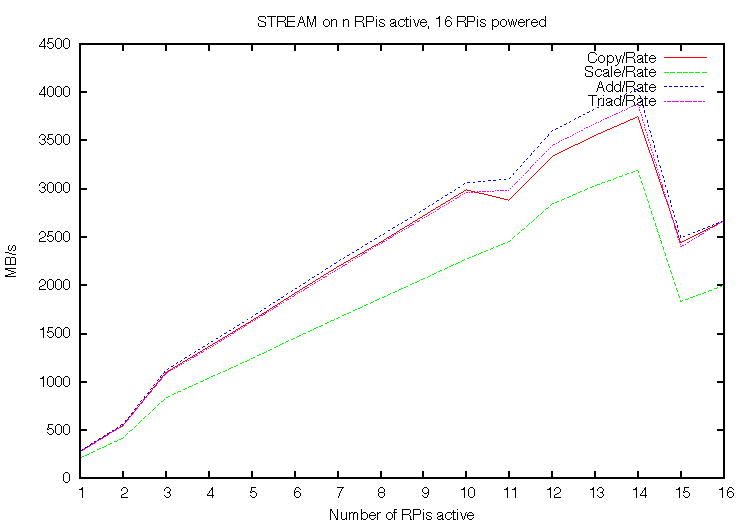
\includegraphics[scale=0.8]{stream1.pdf}\\ 
  \caption{Ausf"uhrungsrate in MB/s f"ur STREAM auf n RPi-Nodes aktiv/16 RPi-Nodes powered.}
  \label{fig:stream1}		
\end{figure}
\begin{figure}[htb]
  \centering
  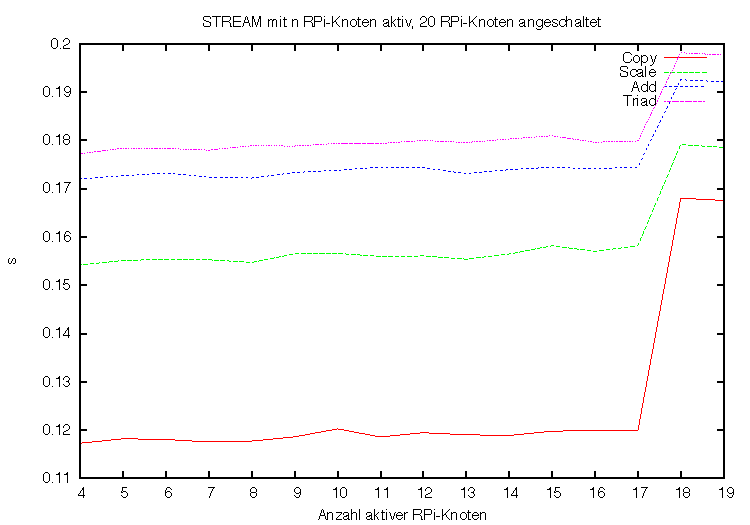
\includegraphics[scale=0.8]{stream2.pdf}\\ 
  \caption{Ausf"uhrungszeit in s f"ur STREAM auf n RPi-Nodes aktiv/16 RPi-Nodes powered.}
  \label{fig:stream2}		
\end{figure}
\begin{figure}[htb]
  \centering
  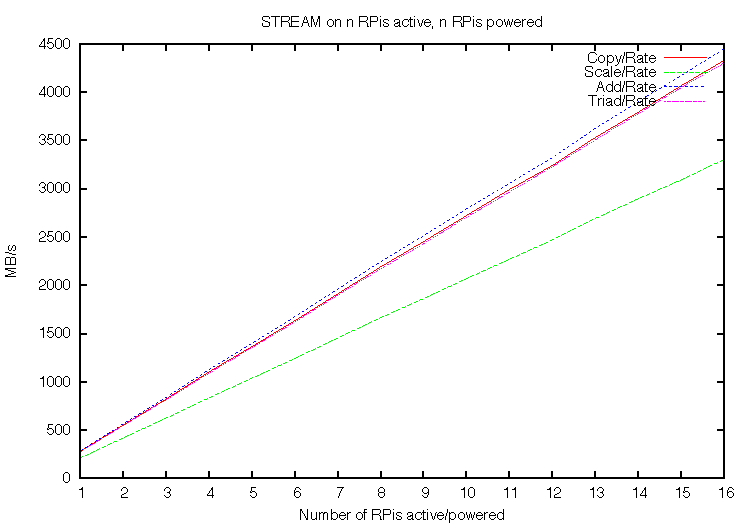
\includegraphics[scale=0.8]{stream3.pdf}\\ 
  \caption{Ausf"uhrungsrate in MB/s f"ur STREAM auf n RPi-Nodes aktiv/n RPi-Nodes powered.}
  \label{fig:stream3}		
\end{figure}
\begin{figure}[htb]
  \centering
  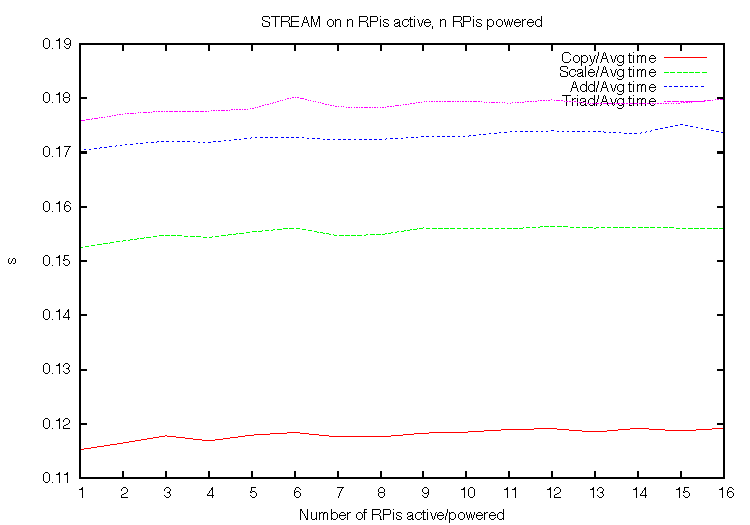
\includegraphics[scale=0.8]{stream4.pdf}\\ 
  \caption{Ausf"uhrungszeit in s f"ur STREAM auf n RPi-Nodes aktiv/n RPi-Nodes powered.}
  \label{fig:stream4}		
\end{figure}

\endinput 


